\chapter{Convolution with Infinite End-Points}
\label{chp:16cases}


\begin{table}[h]
\caption[Possible combinations of finite and infinite end-points]{
	All possible cases of finite and infinite end-points. Finite end-points are denoted with $F$. Infinite left end-points are denoted 	
	$-\infty$ and infinite right end-points are denoted $\infty$.
	\label{fig:16cases}}
\centering
\begin{tabular}{| l || c | c | c | c || r || l ||  c | c | c | c |}
	\hline
		& $a_f$		& $b_f$		& $a_g$		& $b_g$	&$\;\;\;\;$&	& $a_f$		& $b_f$		& $a_g$		& $b_g$	\\
	\hline 
\textit{Case 0:}& $F$	& $F$		& $F$		& $F$	&&	Case 8:	& $-\infty$	& $F$		& $F$		& $F$	\\
Case 1:	& $F$		& $F$		& $F$		& $\infty$&&	Case 9:	& $-\infty$	& $F$		& $F$		& $\infty$ \\
Case 2:	& $F$		& $F$		& $-\infty$	& $F$	&&	Case 10:	& $-\infty$	& $F$		& $-\infty$	& $F$	\\
Case 3:	& $F$		& $F$		& $-\infty$	& $\infty$&&	Case 11:	& $-\infty$	& $F$		& $-\infty$	& $\infty$ \\
Case 4:	& $F$		& $\infty$	& $F$		& $F$	&&	Case 12:	& $-\infty$	& $\infty$	& $F$		& $F$	\\
Case 5:	& $F$		& $\infty$ 	& $F$		& $\infty$&&	Case 13:	& $-\infty$	& $\infty$ 	& $F$		& $\infty$ \\
Case 6:	& $F$		& $\infty$ 	& $-\infty$	& $F$	&&	Case 14:	& $-\infty$	& $\infty$ 	& $-\infty$	& $F$	\\
Case 7:	& $F$		& $\infty$ 	& $-\infty$	& $\infty$&&	Case 15:	& $-\infty$	& $\infty$ 	& $-\infty$	& $\infty$ \\
	\hline
\end{tabular}
\end{table}


When convolving one-piece functions with infinite end-points, there are 4 end-points which can each be either finite or infinite.
As such there are $2^4$ possible combinations of end-point types shown in the table above.
Throughout all calculations in this section, the integrands will not change, only the domains.
So we define the function $\C$ as a sort of restricted convolution:
\begin{equation}
	\C[ [\![x,y)\!) ](t) = \int_{[\![x,y)\!)} f(\tau) g(t-\tau) \; d\tau
\end{equation}
Which can be used to condense equation~(\ref{eqn:defHConvolution}), the definition for hybrid convolution, into:
\begin{align*}
	\label{eqn:defHConvolution2}
	(f^{[a_f,b_f)} \;*\; g^{[a_g,b_g)})
		= \R[+] &\left( \; 
			{\C[ [\![a_f,\;t-a_g)\!) ]}^{[\![a_f+a_g,\; b_f+a_g)\!)} \oplus
			{\C[ [\![a_f,\;b_f)\!) ]}^{[\![b_f+a_g,\; a_f+b_g)\!)} \oplus
			{\C[ [\![t-b_g,\;b_f)\!) ]}^{[\![a_f+b_g,\; b_f+b_g)\!)} 
		\; \right)
\end{align*}


%%%%%%%%%%%%%%%%%%%%%%%%%%%%%%%%%%%%%%%%%
\textbf{Case 0} has all finite points and was already shown to be correct in Section~\ref{sec:HFConvolution} but is listed
for completeness.
The exposition will not be repeated here.


%%%%%%%%%%%%%%%%%%%%%%%%%%%%%%%%%%%%%%%%%
\textbf{Case 1} has one infinite point, $b_g = \infty$ and results in an empty interval for the third term.
Since it is impossible for $t$ to be in $[\![\infty, \infty )\!)$, we can safely remove this term altogether.
\begin{align*}
	(f^{[a_f,b_f)} \;*\; g^{[a_g,\infty)})
	= \R[+] &\left( \;
			{\C[ [\![a_f,\;t-a_g)\!) ]}^{[\![a_f+a_g,\; b_f+a_g)\!)} \oplus
			{\C[ [\![a_f,\;b_f)\!) ]}^{[\![b_f+a_g,\; \infty)\!)} \oplus
			{\C[ [\![-\infty,\;b_f)\!) ]}^{[\![\infty,\; \infty)\!)} 
		\; \right)\\
	= \R[+] &\left( \;
			{\C[ [\![a_f,\;t-a_g)\!) ]}^{[\![a_f+a_g,\; b_f+a_g)\!)} \oplus
			{\C[ [\![a_f,\;b_f)\!) ]}^{[\![b_f+a_g,\; \infty)\!)}
		\; \right)
\end{align*}


Throughout this section we will use sets of diagrams like the one below to verify that our expressions are sensible.
The region where the intervals, $[a_f, b_f)$ and $[t-b_g, t-a_g)$ overlap, (shaded in gray) is where the convolution 
will be non-zero.
The bounds of this intersection may depend on $t$; each case that results in a non-empty intersection will be
shown separately.
To verify an expression, each diagram should correspond to a term in the convolution and the bounds of the shaded 
region should correspond to the domain on that term's integral.
\begin{figure}[h]
	\centering
	\begin{subfigure}[h]{0.4\textwidth}
		\caption{$t \in [\![a_f+a_g, \; b_f+a_g)\!)$} 
		\centering
		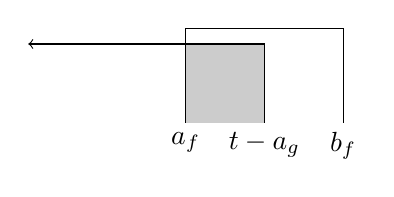
\begin{tikzpicture}
			\draw[fill, color=black!20] (0,0) rectangle (1,1);
			\draw[->] 
				(1,0) node[below](ag){$t-a_g$} 
				-- (1,1) 
				-- (-2,1);
			\draw 
				(0,0) node[below](af){$a_f$} 
				-- (0,1.2) 
				-- (2,1.2) 
				-- (2,0) node[below](bf){$b_f$};
		\end{tikzpicture}
	\end{subfigure}
	\begin{subfigure}[h]{0.4\textwidth}
		\caption{$t \in [\![b_f+a_g, \infty)\!)$} 
		\centering
		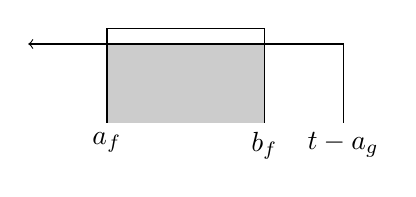
\begin{tikzpicture}
			\draw[fill, color=black!20] (0,0) rectangle (2,1);
			\draw[->] 
				(3,0) node[below](ag){$t-a_g$} 
				-- (3,1) 
				-- (-1,1);
			\draw 
				(0,0) node[below](af){$a_f$} 
				-- (0,1.2) 
				-- (2,1.2) 
				-- (2,0) node[below](bf){$b_f$};
		\end{tikzpicture}
	\end{subfigure}
\end{figure}


%%%%%%%%%%%%%%%%%%%%%%%%%%%%%%%%%%%%%%%%%
\textbf{Case 2} also has only one infinite point, $a_g=-\infty$ and also yields an empty interval:
\begin{align*}
	(f^{[a_f,b_f)} \;*\; g^{[-\infty,b_g)}) 
	= \R[+] &\left( \; 
			{\C[ [\![a_f,\;\infty)\!) ]}^{[\![-\infty,\; -\infty)\!)} \oplus
			{\C[ [\![a_f,\;b_f)\!) ]}^{[\![-\infty,\; a_f+b_g)\!)} \oplus
			{\C[ [\![t-b_g,\;b_f)\!) ]}^{[\![a_f+b_g,\; b_f+b_g)\!)} 
		\; \right)\\
	= \R[+] &\left( \; 
			{\C[ [\![a_f,\;b_f)\!) ]}^{[\![-\infty,\; a_f+b_g)\!)} \oplus
			{\C[ [\![t-b_g,\;b_f)\!) ]}^{[\![a_f+b_g,\; b_f+b_g)\!)} 
		\; \right)
\end{align*} 
\vspace{-1cm}
\begin{figure}[h]
	\centering
	\begin{subfigure}{0.4\textwidth}
		\caption{$t \in [\![-\infty, \; a_f+b_g)\!)$} 
		\centering
		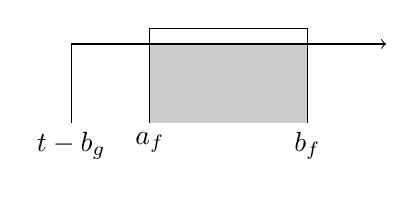
\begin{tikzpicture}
			\draw[fill, color=black!20] (0,0) rectangle (2,1);
			\draw[->] 
				(-1,0) node[below](ag){$t-b_g$} 
				-- (-1,1) 
				-- (3,1);
			\draw 
				(0,0) node[below](af){$a_f$} 
				-- (0,1.2) 
				-- (2,1.2) 
				-- (2,0) node[below](bf){$b_f$};
		\end{tikzpicture}
	\end{subfigure}
	\begin{subfigure}{0.4\textwidth}
		\caption{$t \in [\![a_f+b_g, b_f+b_g)\!)$} 
		\centering
		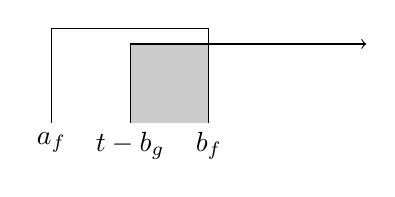
\begin{tikzpicture}
			\draw[fill, color=black!20] (1,0) rectangle (2,1);
			\draw[->] 
				(1,0) node[below](ag){$t-b_g$} 
				-- (1,1) 
				-- (4,1);
			\draw 
				(0,0) node[below](af){$a_f$} 
				-- (0,1.2) 
				-- (2,1.2) 
				-- (2,0) node[below](bf){$b_f$};
		\end{tikzpicture}
	\end{subfigure}
\end{figure}

\pagebreak
%%%%%%%%%%%%%%%%%%%%%%%%%%%%%%%%%%%%%%%%%
\textbf{Case 3} is a combination of both case 1 and 2, resulting in only a single term for the entire real line since
both the first and third terms are over empty intervals.
\begin{align*}
	(f^{[a_f,b_f)} \;*\; g^{[-\infty, \infty)})
	= \R[+] &\left( \; 
			{\C[ [\![a_f,\;\infty)\!) ]}^{[\![-\infty,\; -\infty)\!)} \oplus
			{\C[ [\![a_f,\;b_f)\!) ]}^{[\![-\infty,\; \infty)\!)} \oplus
			{\C[ [\![-\infty,\;b_f)\!) ]}^{[\![\infty,\; \infty)\!)} 
		\; \right) \\
	= \R[+] &\left( \; 
			{\C[ [\![a_f,\;b_f)\!) ]}^{[\![-\infty,\; \infty)\!)} 
		\;\right) 
		=\int_{[\![a_f,\;b_f)\!)} f(\tau) \; g(t-\tau) \; d\tau
\end{align*}
\vspace{-1.5cm}
\begin{figure}[h]
	\centering
	\begin{subfigure}[h]{0.4\textwidth}
		\caption{$t \in [\![-\infty, \; \infty)\!)$} 
		\centering
		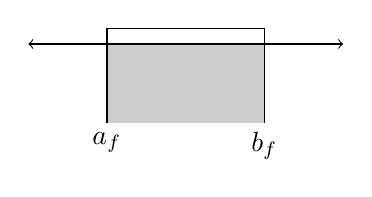
\begin{tikzpicture}
			\draw[fill, color=black!20] (0,0) rectangle (2,1);
			\draw[<->] 
				(-1,1)
				-- (3,1);
			\draw 
				(0,0) node[below](af){$a_f$} 
				-- (0,1.2) 
				-- (2,1.2) 
				-- (2,0) node[below](bf){$b_f$};
		\end{tikzpicture}
	\end{subfigure}
\end{figure}


%%%%%%%%%%%%%%%%%%%%%%%%%%%%%%%%%%%%%%%%%
\textbf{Case 4} (i.e. $b_f = \infty$) is a bit more involved:
\begin{align*}
	(f^{[a_f,\infty)} \;*\; g^{[-\infty,b_g)}) 
	= \R[+] &\left( \; 
			{\C[ [\![a_f,\;t-a_g)\!) ]}^{[\![a_f+a_g,\; \infty)\!)} \oplus
			{\C[ [\![a_f,\;\infty)\!) ]}^{[\![\infty,\; a_f+b_g)\!)} \oplus
			{\C[ [\![t-b_g,\;\infty)\!) ]}^{[\![a_f+b_g,\; \infty)\!)} 
		\; \right) \\
	= \R[+] &\left( \; 
			{\C[ [\![a_f,\;t-a_g)\!) ]}^{[\![a_f+a_g,\; a_f+b_g)\!) \oplus[\![a_f+b_g,\; \infty)\!)} \ominus
			{\C[ [\![a_f,\;\infty)\!) ]}^{[\![a_f+b_g,\; \infty)\!)} \oplus
			{\C[ [\![t-b_g,\;\infty)\!) ]}^{[\![a_f+b_g,\; \infty)\!)} 
		\; \right) \\
	= \R[+] &\left( \; 
			{\C[ [\![a_f,\;t-a_g)\!) ]}^{[\![a_f+a_g,\; a_f+b_g)\!)} \oplus
			{\C[ [\![a_f,\;t-a_g)\!) \ominus [\![a_f,\;\infty)\!) \oplus [\![t-b_g,\;\infty)\!)  ]}^{[\![a_f+b_g,\; \infty)\!)} 
		\; \right) \\
	= \R[+] &\left( \; 
			{\C[ [\![a_f,\;t-a_g)\!) ]}^{[\![a_f+a_g,\; a_f+b_g)\!)} \oplus
			{\C[ [\![t-b_g,\;t-a_g)\!)  ]}^{[\![a_f+b_g,\; \infty)\!)} 
		\; \right)
\end{align*}
\vspace{-1.5cm}
\begin{figure}[h]
	\centering
	\begin{subfigure}[h]{0.4\textwidth}
		\caption{$t \in [\![a_f+a_g, a_f+b_g)\!)$} 
		\centering
		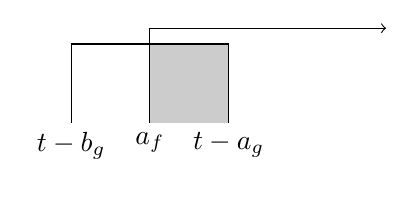
\begin{tikzpicture}
			\draw[fill, color=black!20] (1,0) rectangle (2,1);
			\draw 
				(0,0) node[below](ag){$t-b_g$} 
				-- (0,1) 
				-- (2,1)
				-- (2,0) node[below](af){$t-a_g$};
			\draw[->] 
				(1,0) node[below](af){$a_f$} 
				-- (1,1.2) 
				-- (4,1.2);
		\end{tikzpicture}
	\end{subfigure}
	\begin{subfigure}[h]{0.4\textwidth}
		\caption{$t \in [\![a_f+b_g, \infty)\!)$} 
		\centering
		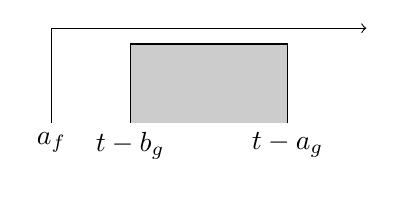
\begin{tikzpicture}
			\draw[fill, color=black!20] (0,0) rectangle (2,1);
			\draw
				(0,0) node[below](bg){$t-b_g$} 
				-- (0,1) 
				-- (2,1)
				-- (2,0) node[below](ag){$t-a_g$};
			\draw[->]
				(-1,0) node[below](af){$a_f$} 
				-- (-1,1.2) 
				-- (3,1.2);
		\end{tikzpicture}
	\end{subfigure}
\end{figure}

%%%%%%%%%%%%%%%%%%%%%%%%%%%%%%%%%%%%%%%%%
\textbf{Case 5} $b_f =\infty$, $b_g = \infty$
\begin{align*}
	(f^{[a_f,\infty)} \;*\; g^{[a_g,\infty)})
		= \R[+] &\left( \; 
			{\C[ [\![a_f,\;t-a_g)\!) ]}^{[\![a_f+a_g,\; \infty)\!)} \oplus
			{\C[ [\![a_f,\;\infty)\!) ]}^{[\![\infty,\; \infty)\!)} \oplus
			{\C[ [\![-\infty,\; \infty)\!) ]}^{[\![\infty,\; \infty)\!)} 
		\; \right)\\
		=\R[+] &\left( \; 
			{\C[ [\![a_f,\;t-a_g)\!) ]}^{[\![a_f+a_g,\; \infty)\!)}
		\; \right)
\end{align*}
\vspace{-1.5cm}
\begin{figure}[h]
	\centering
	\begin{subfigure}[h]{0.4\textwidth}
		\caption{$t \in [\![a_f+a_g, \; \infty)\!)$} 
		\centering
		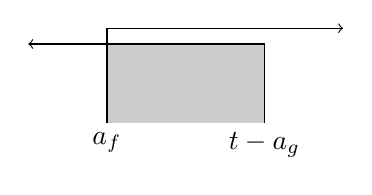
\begin{tikzpicture}
			\draw[fill, color=black!20] (0,0) rectangle (2,1);
			\draw[->] 
				(2,0) node[below](ag){$t-a_g$}
				-- (2,1)
				-- (-1,1);
			\draw[->]
				(0,0) node[below](af){$a_f$} 
				-- (0,1.2) 
				-- (3,1.2);
		\end{tikzpicture}
	\end{subfigure}
\end{figure}

%%%%%%%%%%%%%%%%%%%%%%%%%%%%%%%%%%%%%%%%%
\textbf{Case 6:} $b_f=\infty$, $a_g =-\infty$
\begin{align*}
	(f^{[a_f,\infty)} \;*\; g^{[-\infty,b_g)})
	= \R[+] &\left( \; 
			{\C[ [\![a_f,\;\infty)\!) ]}^{[\![-\infty,\; \bot)\!)} \oplus
			{\C[ [\![a_f,\;\infty)\!) ]}^{[\![\bot,\; a_f+b_g)\!)} \oplus
			{\C[ [\![t-b_g,\;\infty)\!) ]}^{[\![a_f+b_g,\;\infty)\!)} 
		\; \right) \\
	= \R[+] &\left( \; 
			{\C[ [\![a_f,\;\infty)\!) ]}^{[\![-\infty,\; a_f+b_g)\!)} \oplus
			{\C[ [\![t-b_g,\;\infty)\!) ]}^{[\![a_f+b_g,\;\infty)\!)} 
		\; \right)
\end{align*}
\vspace{-1.5cm}
\begin{figure}[h]
	\centering
	\begin{subfigure}[h]{0.4\textwidth}
		\caption{$t \in [\![-\infty, a_f+b_g)\!)$} 
		\centering
		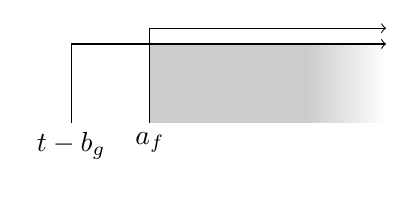
\begin{tikzpicture}
			\draw[fill, color=black!20] (1,0) rectangle (3,1);
			\shade[left color=black!20, right color=white] (3,0) rectangle (4,1);
			\draw[->]
				(0,0) node[below](bg){$t-b_g$} 
				-- (0,1) 
				-- (4,1);
			\draw[->] 
				(1,0) node[below](af){$a_f$} 
				-- (1,1.2) 
				-- (4,1.2);
		\end{tikzpicture}
	\end{subfigure}
	\begin{subfigure}[h]{0.4\textwidth}
		\caption{$t \in [\![a_f+b_g, \infty)\!)$} 
		\centering
		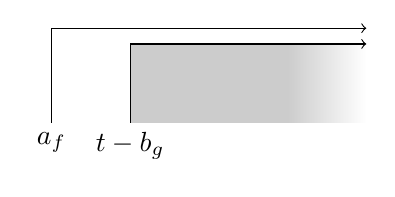
\begin{tikzpicture}
			\draw[fill, color=black!20] (1,0) rectangle (3,1);
			\shade[left color=black!20, right color=white] (3,0) rectangle (4,1);
			\draw[->]
				(1,0) node[below](bg){$t-b_g$} 
				-- (1,1) 
				-- (4,1);
			\draw[->] 
				(0,0) node[below](af){$a_f$} 
				-- (0,1.2) 
				-- (4,1.2);
		\end{tikzpicture}
	\end{subfigure}
\end{figure}

%%%%%%%%%%%%%%%%%%%%%%%%%%%%%%%%%%%%%%%%%
\textbf{Case 7:} $b_f=\infty$, $a_g =-\infty$, $b_g=\infty$
\begin{align*}
	(f^{[a_f,\infty)} \;*\; g^{[-\infty,\infty)})
	= \R[+] &\left( \; 
			{\C[ [\![a_f,\;\infty)\!) ]}^{[\![-\infty,\; \bot)\!)} \oplus
			{\C[ [\![a_f,\;\infty)\!) ]}^{[\![\bot,\; \infty)\!)} \oplus
			{\C[ [\![-\infty,\;\infty)\!) ]}^{[\![\infty,\; \infty)\!)} 
		\; \right) \\
	= \R[+] &\left( \; 
			{\C[ [\![a_f,\;\infty)\!) ]}^{[\![-\infty,\; \infty)\!)}
		\; \right)
\end{align*}
\vspace{-1.5cm}
\begin{figure}[h]
	\centering
	\begin{subfigure}[h]{0.4\textwidth}
		\caption{$t \in [\![-\infty, \; \infty)\!)$} 
		\centering
		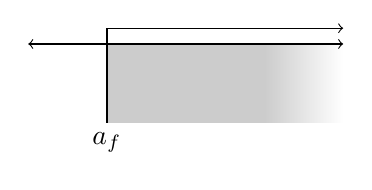
\begin{tikzpicture}
			\draw[fill, color=black!20] (0,0) rectangle (2,1);
			\shade[left color=black!20, right color=white] (2,0) rectangle (3,1);
			\draw[<->] 
				(-1,1)
				-- (3,1);
			\draw[->]
				(0,0) node[below](af){$a_f$} 
				-- (0,1.2) 
				-- (3,1.2);
		\end{tikzpicture}
	\end{subfigure}
\end{figure}


%%%%%%%%%%%%%%%%%%%%%%%%%%%%%%%%%%%%%%%%%
\textbf{Case 8:} $a_f=-\infty$
\begin{align*}
	(f^{[-\infty,b_f)} \;*\; g^{[a_g,b_g)})
	= \R[+] &\left( \; 
			{\C[ [\![-\infty,\;t-a_g)\!) ]}^{[\![-\infty,\; b_f+a_g)\!)} \oplus
			{\C[ [\![-\infty,\;b_f)\!) ]}^{[\![b_f+a_g,\; -\infty)\!)} \oplus
			{\C[ [\![t-b_g,\;b_f)\!) ]}^{[\![-\infty,\; b_f+b_g)\!)} 
		\; \right) \\	
	= \R[+] &\left( \; 
			{\C[ [\![-\infty,\;t-a_g)\!) ]}^{[\![-\infty,\; b_f+a_g)\!)} \ominus
			{\C[ [\![-\infty,\;b_f)\!) ]}^{[\![-\infty, \; b_f+a_g)\!)} \oplus
			{\C[ [\![t-b_g,\;b_f)\!) ]}^{[\![-\infty,\; b_f+a_g)\!)\oplus[\![b_f+a_g, b_f+b_g)\!)} 
		\; \right) \\
	= \R[+] &\left( \; 
			{\C[ [\![-\infty,\;t-a_g)\!)
				\ominus[\![-\infty,\;b_f)\!)
				\oplus[\![t-b_g,\;b_f)\!) ]}^{[\![-\infty,\; b_f+a_g)\!)} \oplus
			{\C[ [\![t-b_g,\;b_f)\!) ]}^{[\![b_f+a_g, b_f+b_g)\!)} 
		\; \right) \\
	= \R[+] &\left( \; 
			{\C[ [\![t-b_g,\;t-a_g)\!) ]}^{[\![-\infty,\; b_f+a_g)\!)} \oplus
			{\C[ [\![t-b_g,\;b_f)\!) ]}^{[\![b_f+a_g, b_f+b_g)\!)} 
		\; \right)
\end{align*}
\vspace{-1.5cm}
\begin{figure}[h]
	\centering
	\begin{subfigure}[h]{0.4\textwidth}
		\caption{$t \in [\![-\infty, b_f+a_g)\!)$} 
		\centering
		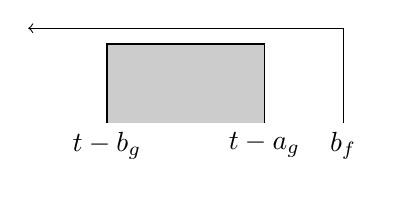
\begin{tikzpicture}
			\draw[fill, color=black!20] (0,0) rectangle (2,1);
			\draw[->] 
				(3,0) node[below](bf){$b_f$} 
				-- (3,1.2) 
				-- (-1,1.2);
			\draw 
				(0,0) node[below](bg){$t-b_g$} 
				-- (0,1) 
				-- (2,1) 
				-- (2,0) node[below](ag){$t-a_g$};
		\end{tikzpicture}
	\end{subfigure}
	\begin{subfigure}[h]{0.4\textwidth}
		\caption{$t \in [\![b_f+a_g, b_f+b_g)\!)$} 
		\centering
		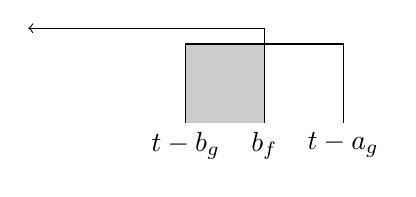
\begin{tikzpicture}
			\draw[fill, color=black!20] (0,0) rectangle (1,1);
			\draw 
				(0,0) node[below](bg){$t-b_g$} 
				-- (0,1) 
				-- (2,1) 
				-- (2,0) node[below](ag){$t-a_g$};
			\draw[->] 
				(1,0) node[below](bf){$b_f$} 
				-- (1,1.2) 
				-- (-2,1.2);
		\end{tikzpicture}
	\end{subfigure}
\end{figure}


%%%%%%%%%%%%%%%%%%%%%%%%%%%%%%%%%%%%%%%%%
\textbf{Case 9:} $a_f=-\infty$, $b_g=\infty$
\begin{align*}
	(f^{[-\infty,b_f)} \;*\; g^{[a_g,\infty)})
	= \R[+] &\left( \; 
			{\C[ [\![-\infty,\;t-a_g)\!) ]}^{[\![-\infty,\; b_f+a_g)\!)} \oplus
			{\C[ [\![-\infty,\;b_f)\!) ]}^{[\![b_f+a_g,\; \bot)\!)} \oplus
			{\C[ [\![-\infty,\;b_f)\!) ]}^{[\![\bot,\;\infty)\!)} 
		\; \right) \\
	= \R[+] &\left( \; 
			{\C[ [\![-\infty,\;t-a_g)\!) ]}^{[\![-\infty,\; b_f+a_g)\!)} \oplus
			{\C[ [\![-\infty,\;b_f)\!) ]}^{[\![b_f+a_g,\; \infty)\!)}
		\; \right) 
\end{align*}
\vspace{-1.5cm}
\begin{figure}[h]
	\centering
	\begin{subfigure}[h]{0.4\textwidth}
		\caption{$t \in [\![-\infty, b_f+a_g)\!)$} 
		\centering
		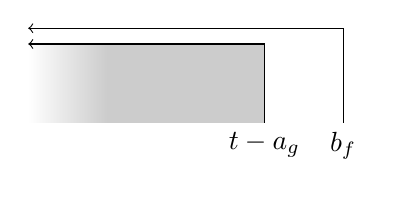
\begin{tikzpicture}
			\draw[fill, color=black!20] (0,0) rectangle (2,1);
			\shade[right color=black!20, left color=white] (-1,0) rectangle (0,1);
			\draw[->] 
				(3,0) node[below](bf){$b_f$} 
				-- (3,1.2) 
				-- (-1,1.2);
			\draw[->] 
				(2,0) node[below](ag){$t-a_g$}
				-- (2,1)
				-- (-1,1);
		\end{tikzpicture}
	\end{subfigure}
	\begin{subfigure}[h]{0.4\textwidth}
		\caption{$t \in [\![b_f+a_g, \infty)\!)$} 
		\centering
		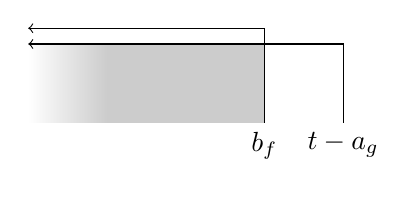
\begin{tikzpicture}
			\draw[fill, color=black!20] (0,0) rectangle (2,1);
			\shade[right color=black!20, left color=white] (-1,0) rectangle (0,1);
			\draw[->] 
				(2,0) node[below](bf){$b_f$} 
				-- (2,1.2) 
				-- (-1,1.2);
			\draw[->] 
				(3,0) node[below](ag){$t-a_g$}
				-- (3,1)
				-- (-1,1);
		\end{tikzpicture}
	\end{subfigure}
\end{figure}

%%%%%%%%%%%%%%%%%%%%%%%%%%%%%%%%%%%%%%%%%
\textbf{Case 10:} $a_f=-\infty$, $a_g =-\infty$
\begin{align*}
	(f^{[-\infty,b_f)} \;*\; g^{[-\infty,b_g)})
	= \R[+] &\left( \; 
			{\C[ [\![-\infty,\;\infty)\!) ]}^{[\![-\infty,\; -\infty)\!)} \oplus
			{\C[ [\![-\infty,\;b_f)\!) ]}^{[\![-\infty,\; -\infty)\!)} \oplus
			{\C[ [\![t-b_g,\;b_f)\!) ]}^{[\![-\infty,\; b_f+b_g)\!)} 
		\; \right) \\ 
	= \R[+] &\left( \; 
			{\C[ [\![t-b_g,\;b_f)\!) ]}^{[\![-\infty,\; b_f+b_g)\!)} 
		\; \right)
\end{align*}
\vspace{-1.5cm}
\begin{figure}[h]
	\centering
	\begin{subfigure}[h]{0.4\textwidth}
		\caption{$t \in [\![-\infty, b_f+b_g)\!)$} 
		\centering
		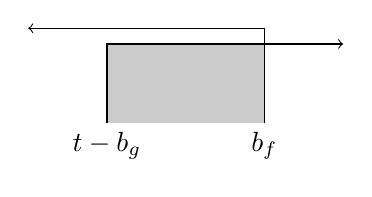
\begin{tikzpicture}
			\draw[fill, color=black!20] (1,0) rectangle (3,1);
			\draw[->] 
				(3,0) node[below](bf){$b_f$} 
				-- (3,1.2) 
				-- (0,1.2);
			\draw[->]
				(1,0) node[below](bg){$t-b_g$} 
				-- (1,1) 
				-- (4,1);
		\end{tikzpicture}
	\end{subfigure}
\end{figure}


%%%%%%%%%%%%%%%%%%%%%%%%%%%%%%%%%%%%%%%%%
\textbf{Case 11:} $a_f=-\infty$, $a_g =-\infty$, $b_g=\infty$
\begin{align*}
	(f^{[-\infty,b_f)} \;*\; g^{[-\infty,\infty)})
	= \R[+] &\left( \; 
			{\C[ [\![-\infty,\;\infty)\!) ]}^{[\![-\infty,\; -\infty)\!)} \oplus
			{\C[ [\![-\infty,\;b_f)\!) ]}^{[\![-\infty,\; \bot)\!)} \oplus
			{\C[ [\![-\infty,\;b_f)\!) ]}^{[\![\bot,\; \infty)\!)} 
		\; \right) \\ 
	= \R[+] &\left( \; 
			{\C[ [\![-\infty,\;b_f)\!) ]}^{[\![-\infty,\; \infty)\!)}
		\; \right)
\end{align*}
\vspace{-1.5cm}
\begin{figure}[h]
	\centering
	\begin{subfigure}[h]{0.4\textwidth}
		\caption{$t \in [\![-\infty, \infty)\!)$} 
		\centering
		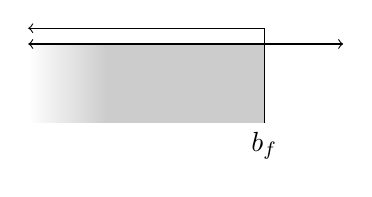
\begin{tikzpicture}
			\draw[fill, color=black!20] (0,0) rectangle (2,1);
			\shade[right color=black!20, left color=white] (-1,0) rectangle (0,1);
			\draw[->] 
				(2,0) node[below](bf){$b_f$} 
				-- (2,1.2) 
				-- (-1,1.2);
			\draw[<->] 
				(3,1)
				-- (-1,1);
		\end{tikzpicture}
	\end{subfigure}
\end{figure}


%%%%%%%%%%%%%%%%%%%%%%%%%%%%%%%%%%%%%%%%%
\textbf{Case 12:} $a_f=-\infty$, $b_f=\infty$
\begin{align*}
	(f^{[-\infty,\infty)} \;*\; g^{[a_g,b_g)})
	= \R[+] &\left( \; 
			{\C[ [\![-\infty,\;t-a_g)\!) ]}^{[\![-\infty,\;\infty)\!)} \oplus
			{\C[ [\![-\infty,\;\infty)\!) ]}^{[\![\infty,\; -\infty)\!)} \oplus
			{\C[ [\![t-b_g,\;\infty)\!) ]}^{[\![-\infty,\; \infty)\!)} 
		\; \right) \\
	= \R[+] &\left( \; 
			{\C[ [\![-\infty,\;t-a_g)\!)\ominus[\![-\infty,\;\infty)\!)\oplus[\![t-b_g,\;\infty)\!) ]}^{[\![-\infty,\;\infty)\!)}
		\; \right) \\
	= \R[+] &\left( \; 
			{\C[ [\![[t-b_g,\;t-a_g)\!) ]}^{[\![-\infty,\;\infty)\!)}
		\; \right) \\
\end{align*}
\vspace{-3cm}
\begin{figure}[h]
	\centering
	\begin{subfigure}[h]{0.4\textwidth}
		\caption{$t \in [\![-\infty, \; \infty)\!)$} 
		\centering
		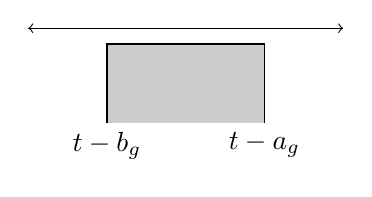
\begin{tikzpicture}
			\draw[fill, color=black!20] (0,0) rectangle (2,1);
			\draw[<->] 
				(-1,1.2)
				-- (3,1.2);
			\draw 
				(0,0) node[below](bg){$t-b_g$} 
				-- (0,1) 
				-- (2,1) 
				-- (2,0) node[below](ag){$t-a_g$};
		\end{tikzpicture}
	\end{subfigure}
\end{figure}



%%%%%%%%%%%%%%%%%%%%%%%%%%%%%%%%%%%%%%%%%
\textbf{Case 13:} $a_f=-\infty$, $b_f=\infty$, $b_g=\infty$
\begin{align*}
	(f^{[-\infty,\infty)} \;*\; g^{[a_g,\infty)})
	= \R[+] &\left( \; 
			{\C[ [\![-\infty,\;t-a_g)\!) ]}^{[\![-\infty,\; \infty)\!)} \oplus
			{\C[ [\![-\infty,\;\infty)\!) ]}^{[\![\infty,\; \bot)\!)} \oplus
			{\C[ [\![-\infty,\;\infty)\!) ]}^{[\![\bot,\; \infty)\!)} 
		\; \right) \\
	= \R[+] &\left( \; 
			{\C[ [\![-\infty,\;t-a_g)\!) ]}^{[\![-\infty,\; \infty)\!)} \oplus
			{\C[ [\![-\infty,\;\infty)\!) ]}^{[\![\infty,\; \infty)\!)} 
		\; \right) \\
	= \R[+] &\left( \; 
			{\C[ [\![-\infty,\;t-a_g)\!) ]}^{[\![-\infty,\; \infty)\!)}
		\; \right)
\end{align*}
\vspace{-1.5cm}
\begin{figure}[h]
	\centering
	\begin{subfigure}[h]{0.4\textwidth}
		\caption{$t \in [\![-\infty, \; \infty)\!)$} 
		\centering
		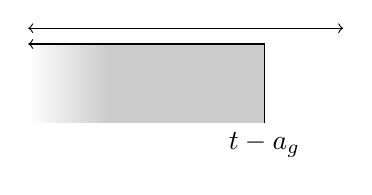
\begin{tikzpicture}
			\draw[fill, color=black!20] (0,0) rectangle (2,1);
			\shade[left color=white, right color=black!20] (-1,0) rectangle (0,1);
			\draw[<->] 
				(-1,1.2)
				-- (3,1.2);
			\draw[<-] 
				(-1,1) 
				-- (2,1) 
				-- (2,0) node[below](ag){$t-a_g$};
		\end{tikzpicture}
	\end{subfigure}
\end{figure}


%%%%%%%%%%%%%%%%%%%%%%%%%%%%%%%%%%%%%%%%%
\textbf{Case 14:} $a_f=-\infty$, $b_f=\infty$, $a_g =-\infty$
\begin{align*}
	(f^{[-\infty,\infty)} \;*\; g^{[-\infty,b_g)})
	= \R[+] &\left( \; 
			{\C[ [\![-\infty,\;\infty)\!) ]}^{[\![-\infty,\; \bot)\!)} \oplus
			{\C[ [\![-\infty,\;\infty)\!) ]}^{[\![\bot,\; -\infty)\!)} \oplus
			{\C[ [\![t-b_g,\;\infty)\!) ]}^{[\![-\infty,\; \infty)\!)} 
		\; \right) \\
	= \R[+] &\left( \; 
			{\C[ [\![-\infty,\;\infty)\!) ]}^{[\![-\infty,\; -\infty)\!)} \oplus
			{\C[ [\![t-b_g,\;\infty)\!) ]}^{[\![-\infty,\; \infty)\!)} 
		\; \right) \\
	= \R[+] &\left( \; 
			{\C[ [\![t-b_g,\;\infty)\!) ]}^{[\![-\infty,\; \infty)\!)} 
		\; \right) 
\end{align*}
\vspace{-1.5cm}
\begin{figure}[h]
	\centering
	\begin{subfigure}[h]{0.4\textwidth}
		\caption{$t \in [\![-\infty, \; \infty)\!)$} 
		\centering
		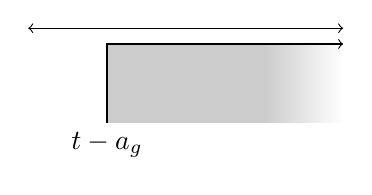
\begin{tikzpicture}
			\draw[fill, color=black!20] (0,0) rectangle (2,1);
			\shade[right color=white, left color=black!20] (2,0) rectangle (3,1);
			\draw[<->] 
				(-1,1.2)
				-- (3,1.2);
			\draw[<-] 
				(3,1) 
				-- (0,1) 
				-- (0,0) node[below](ag){$t-a_g$};
		\end{tikzpicture}
	\end{subfigure}
\end{figure}


%%%%%%%%%%%%%%%%%%%%%%%%%%%%%%%%%%%%%%%%%
\textbf{Case 15:} $a_f=-\infty$, $b_f=\infty$, $a_g =-\infty$, $b_g=\infty$
has all infinite points and is not really what one would think of as a one-piece function at all.
The definition of convolution already holds for such functions.
That being said:
\begin{align*}
	(f^{[-\infty,\infty)} \;*\; g^{[-\infty,\infty)})
	= \R[+] &\left( \; 
			{\C[ [\![-\infty,\;\infty)\!) ]}^{[\![-\infty,\; \bot_1)\!)} \oplus
			{\C[ [\![-\infty,\;\infty)\!) ]}^{[\![\bot_1,\;\bot_2)\!)} \oplus
			{\C[ [\![-\infty,\;\infty)\!) ]}^{[\![\bot_2,\; \infty)\!)} 
		\; \right) \\
	= \R[+] &\left( \; 
			{\C[ [\![-\infty,\;\infty)\!) ]}^{[\![-\infty,\; \infty)\!)} 
		\; \right) \\
	= & \int_{[\![ -\infty, \; \infty )\!)} f(\tau)g(t-\tau) \; d\tau
\end{align*}


\begin{lstlisting}[frame=single, mathescape]
Convolve := proc(f,af,bf,g,ag,bg)
 local afbg,bfag,out,temp;
 if(af+bg != undefined) then afbg := af+bg; fi;
 if(bf+ag != undefined) then bfag := bf+ag; fi;
 out:=(int(fg(x),x=af..t-ag))*(OrientedInterval(af+ag,bfag))(t)
    +(int(fg(x),x=af..bf))*(OrientedInterval(bfag,afbg))(t)
    +(int(fg(x),x=t-bg..bf))*(OrientedInterval(afbg,bf+bg))(t);
 out:=subs(t-infinity=-infinity,out);
 out:=subs(t+infinity=infinity,out);
 try temp := convert(out,piecewise,t);
 catch: 
    try temp:=convert(convert(out,Heaviside),piecewise,t);
    catch: temp := out; end try;  
 finally out := temp; end try;
 try temp := Combine(subs(infinity=infty,out));
    catch temp:=out;
 finally out:=subs(infty=infinity,temp); end try;
 out := subs(fg(x)=f(x)*g(t-x), out);
end proc;
\end{lstlisting}

\begin{mdframed}\begin{lstlisting}[mathescape]
> Convolve(sin, 0, Pi, t->exp(-t), 0, 1);

		$\displaystyle \begin{cases}
	0 & t\!\sim\;<0 \\
	\int_{t\sim}^0 \sin(x)e^{-t\sim+x} \; dx & t\!\sim\;<1 \\
	\int_{-1+t\sim}^{t\sim} \sin(x)e^{-t\sim+x} \; dx & t\!\sim\;<\pi \\
	\int_{-1+t\sim}^{t\sim} \sin(x)e^{-t\sim+x} \; dx & t\!\sim\;<\pi+1 \\
	0 & \pi+1 \leq t\!\sim
	\end{cases}$
\end{lstlisting}
\end{mdframed}

\textbf{Case 1:}

\begin{mdframed}\begin{lstlisting}[ mathescape]
> assume(t::real); additionally(af<bf); additionally(ag<bg);
> Convolve(f,af,bf,g,ag,infinity);

		$\displaystyle \begin{cases}
	0 & t\!\sim\;<af\sim+ag\sim \\
	\int_{af\sim}^{t\sim-ag\sim} f(x)g(t\sim-x) \; dx & t\!\sim\;<bf\sim+ag\sim \\
	\int_{af\sim}^{bf\sim} f(x)g(t\sim-x) \; dx & bf\sim+ag\sim \leq t\sim
	\end{cases}$
\end{lstlisting}
\end{mdframed}


